\chapter{Background}
\label{ch:background}

This chapter establishes the theoretical foundations and contextual literature underpinning the comparative study of PageRank and HITS. We begin with a self-contained presentation of the core concepts (Section~\ref{sec:concepts_overview}), followed by a structured literature review (Section~\ref{sec:literature_review}), a description of the dataset (Section~\ref{sec:datasets}), a definition of evaluation metrics (Section~\ref{sec:eval_metrics_bg}), and a synthesizing discussion (Section~\ref{sec:bg_discussion}).


%=============================================================
\section{Concepts Overview}
\label{sec:concepts_overview}

%-------------------------------------------------------------
\subsection{Link Analysis and Web Graph Theory}
\label{subsec:link_analysis}

The World Wide Web can be formally represented as a directed graph $G = (V, E)$, where the set of vertices $V = \{v_1, v_2, \dots, v_N\}$ corresponds to individual web pages and the set of directed edges $E \subseteq V \times V$ corresponds to hyperlinks. An edge $(u, v) \in E$ indicates that page $u$ contains a hyperlink pointing to page $v$. The \textit{in-degree} of a node $v$, denoted $\deg^{-}(v) = |B(v)|$, is the number of edges directed toward $v$, while the \textit{out-degree}, denoted $\deg^{+}(v) = |F(v)|$, is the number of edges originating from $v$. Here, $B(v) = \{u \in V : (u,v) \in E\}$ denotes the set of \textit{predecessors} (or in-neighbors) and $F(v) = \{w \in V : (v,w) \in E\}$ denotes the set of \textit{successors} (or out-neighbors) of $v$~\cite{brin1998pagerank, stanford1999pagerank}.

Link analysis is the discipline concerned with extracting meaningful structural information---rankings, centrality measures, community structures, and influence flows---from the topology of such directed graphs. The central premise is that the pattern of hyperlinks encodes collective human judgment about the relative importance and relevance of web pages. Two principal algorithmic paradigms have dominated this field: PageRank and HITS, which differ fundamentally in their scope, execution model, and the type of structural information they extract~\cite{kleinberg1999hits, ijarcce_comparative}.


%-------------------------------------------------------------
\subsection{The PageRank Algorithm}
\label{subsec:pagerank}

In 1998, Sergey Brin and Larry Page introduced the PageRank algorithm, fundamentally shifting web search from purely textual matching to structural link analysis. By conceptualizing the World Wide Web as a massive directed graph, PageRank operated on the premise that a hyperlink from one page to another acts as an endorsement. This allowed search engines to rank pages based on their objective, topological authority rather than easily manipulated keyword frequencies, significantly improving the quality of information retrieval~\cite{brin1998pagerank}.

To formalize this model, web pages are conceptualized as nodes in a directed graph, where hyperlinks serve as directed edges, or backlinks. Figure~\ref{fig:web_graph_concept} demonstrates this fundamental structure: a directed hyperlink from Page $A$ to Page $B$ constitutes an endorsement, transferring structural importance to Page $B$. Page $C$ receives multiple incoming edges (backlinks) from other pages, thereby accumulating a higher PageRank score. The visual styling of this network (represented in dark-theme blue accents) mirrors the interactive node-link visualization layout utilized in the backend of the Transfer Analyzer application developed in this thesis.

\begin{figure}[H]
    \centering
    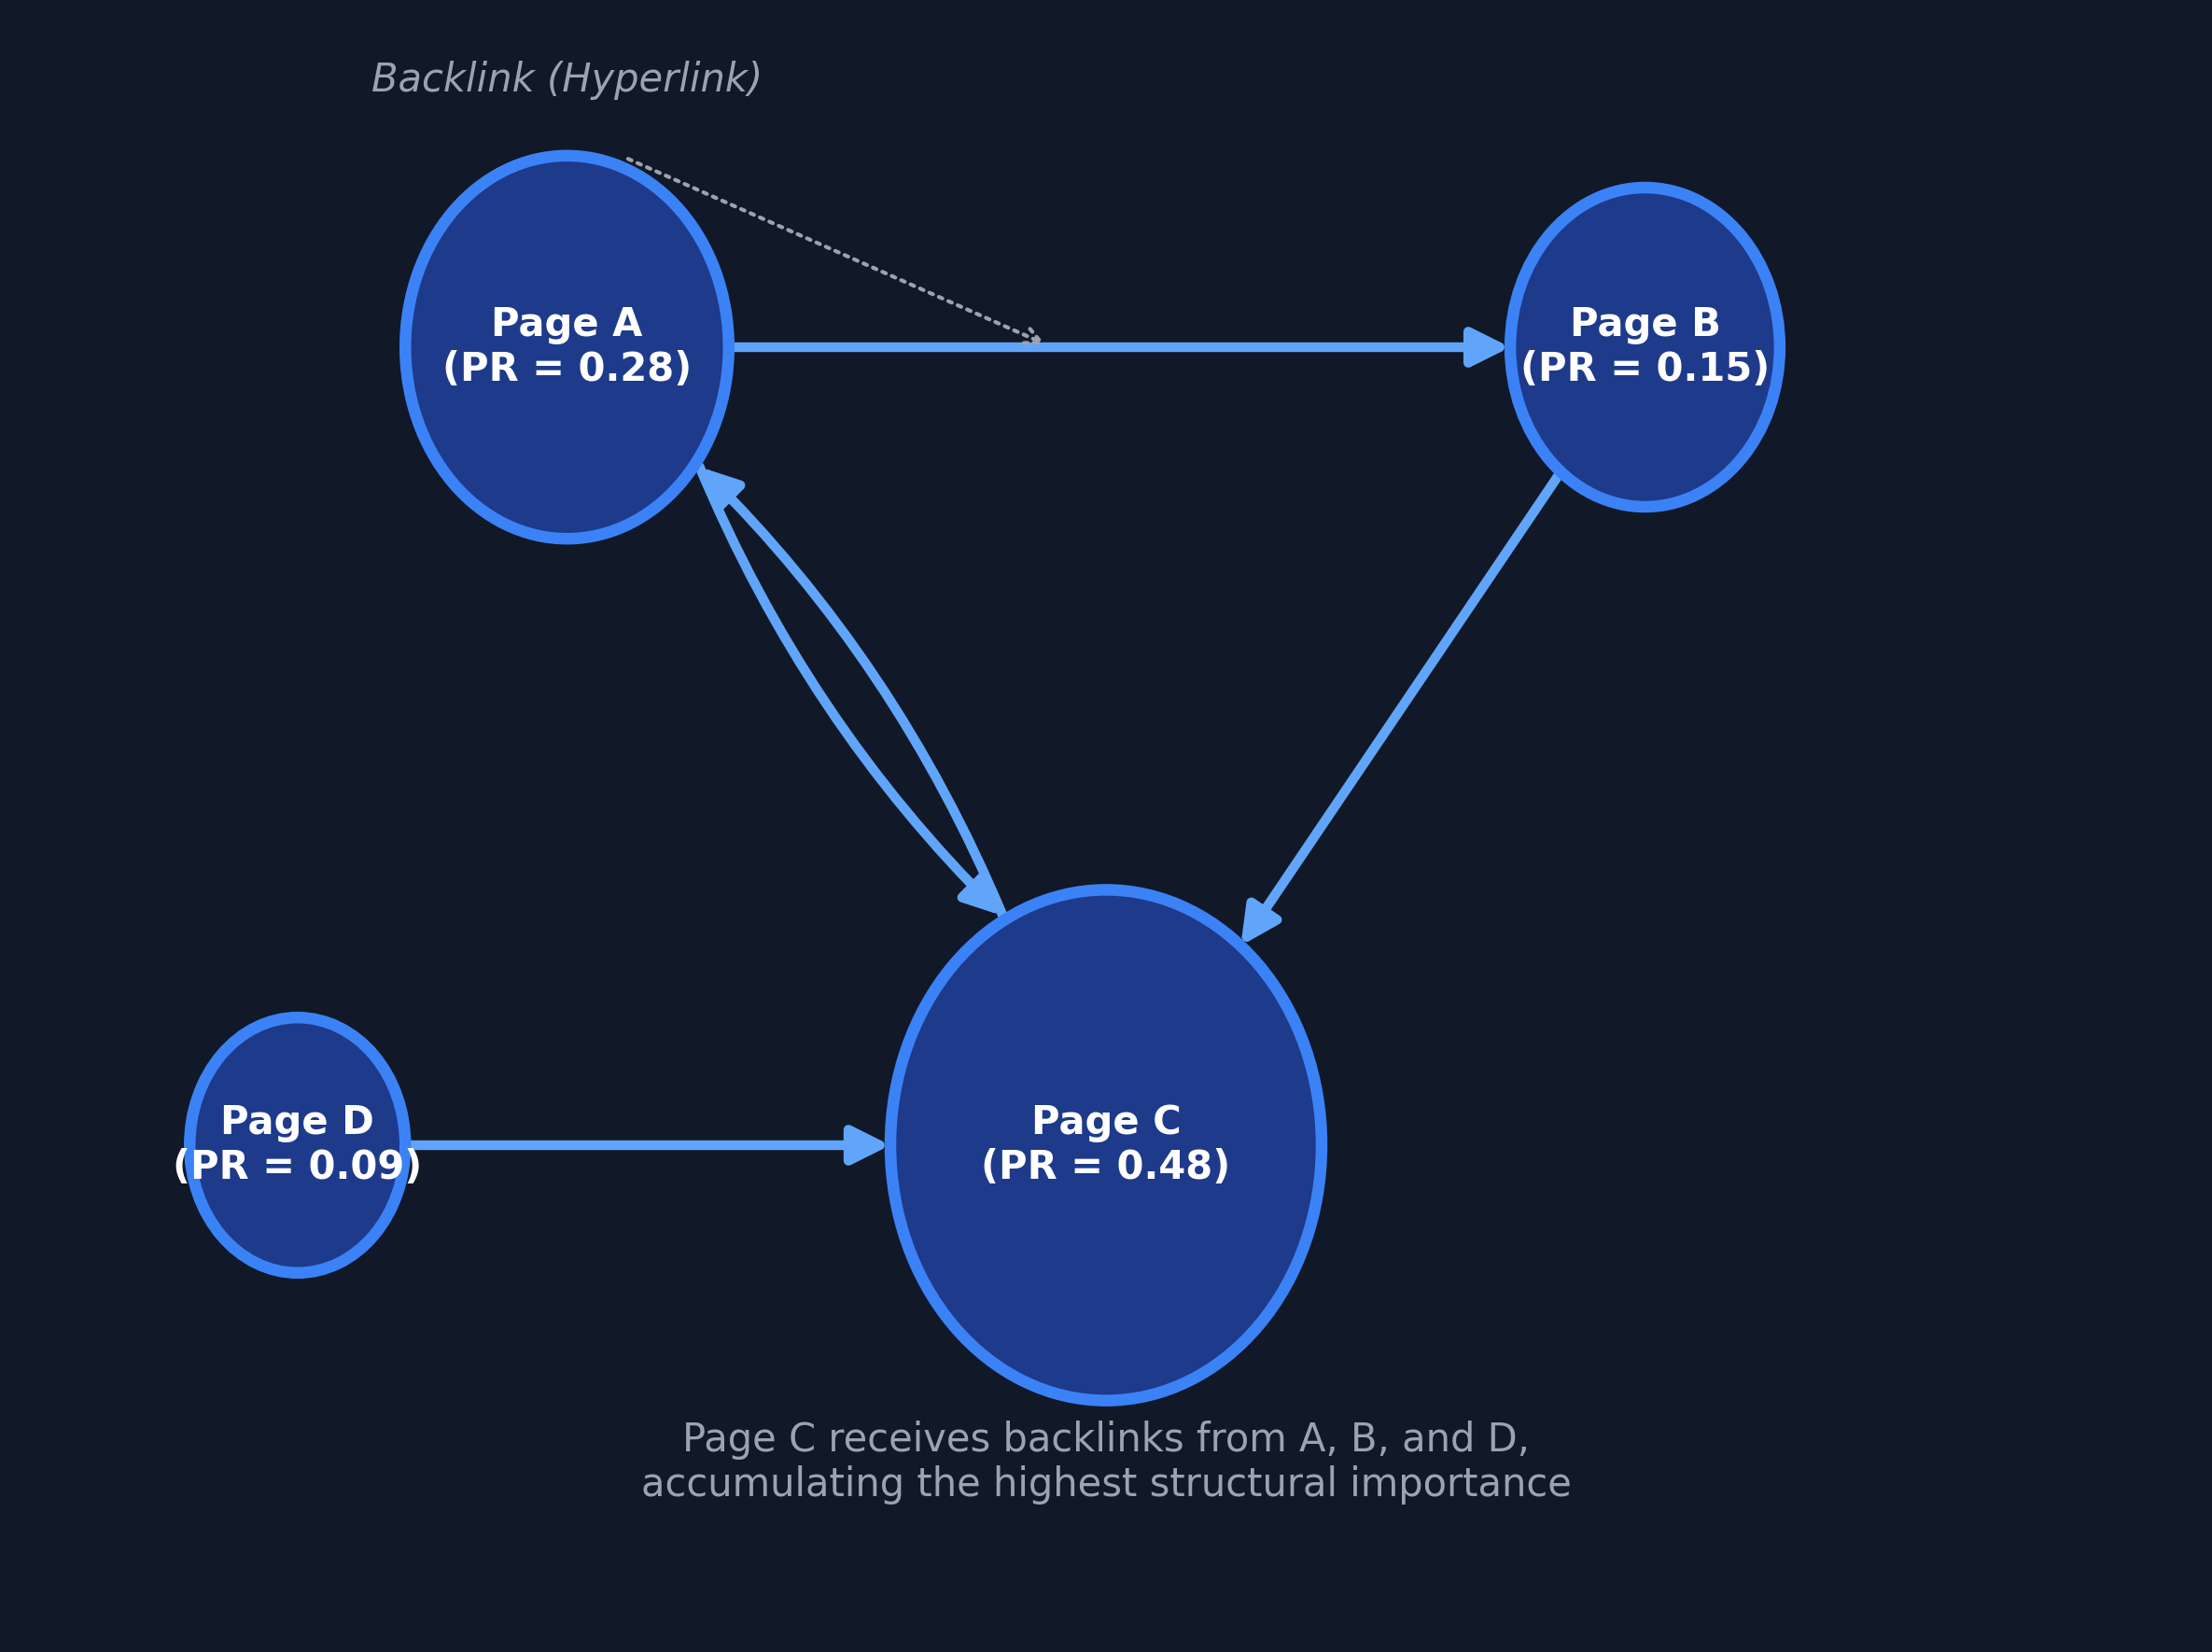
\includegraphics[width=0.8\textwidth]{Figures/web_graph_concept.png}
    \caption{Conceptual diagram of web pages and backlinks modeling structural endorsements.}
    \label{fig:web_graph_concept}
\end{figure}

\subsubsection{The Random Surfer Model and Markov Chains}

Classical PageRank relies on the ``random surfer'' model, simulating a user randomly clicking hyperlinks. Modeled as a directed graph $G=(V,E)$, a node $u$ confers a fraction of its importance, $PR(u)/L(u)$ (where $L(u)$ is the out-degree of $u$), to its destination node $v$. The iterative propagation of rank is defined as:
\begin{equation}
\label{eq:pagerank_basic}
PR_{i+1}(v) = \sum_{u \in B(v)} \frac{PR_{i}(u)}{L(u)}
\end{equation}
where $B(v)$ is the set of all nodes pointing to $v$. This formulation is a discrete-time Markov chain, represented by a transition matrix~\cite{brin1998pagerank, stanford1999pagerank}.

The transition matrix $\mathbf{M}$ of this Markov chain is defined such that the entry $M_{ij} = 1/L(j)$ if there exists an edge from node $j$ to node $i$, and $M_{ij} = 0$ otherwise. The PageRank vector $\boldsymbol{\pi}$ is then the stationary distribution of the Markov chain, satisfying $\boldsymbol{\pi} = \mathbf{M}\boldsymbol{\pi}$---that is, it is the principal eigenvector of $\mathbf{M}$ corresponding to eigenvalue~1~\cite{stanford1999pagerank}.


\subsubsection{Damping Factor and Eigenvector Computation}

To resolve topological anomalies like ``spider traps'' and ``dangling nodes,'' PageRank introduces a damping factor, $d$ (typically 0.85), representing the probability that the surfer follows existing links. With probability $1-d$, the surfer teleports to a random page in the network. The modified formula is:
\begin{equation}
\label{eq:pagerank_damped}
PR(v) = \frac{1-d}{N} + d \sum_{u \in B(v)} \frac{PR(u)}{L(u)}
\end{equation}
This transforms the matrix into a strictly positive Google Matrix, ensuring convergence to a unique principal eigenvector via the power iteration method~\cite{brin1998pagerank, stanford1999pagerank}.

In matrix notation, the Google Matrix $\mathbf{G}$ is defined as:
\begin{equation}
\label{eq:google_matrix}
\mathbf{G} = d\,\mathbf{M} + \frac{1-d}{N}\,\mathbf{1}\mathbf{1}^{T}
\end{equation}
where $\mathbf{1}$ is the $N$-dimensional column vector of ones. By the Perron--Frobenius theorem, since $\mathbf{G}$ is a column-stochastic, primitive, and irreducible matrix, it possesses a unique stationary distribution that the power iteration method is guaranteed to converge to~\cite{stanford1999pagerank, mdpi_gluing}.


\subsubsection{Convergence and Complexity}

The algorithm's convergence rate is bounded by the damping factor $d$. The overall time complexity for computation via the power method is $O(k \times (N + E))$, where $N$ represents nodes, $E$ represents edges, and $k$ represents the iterations required, making it highly scalable for large graphs~\cite{brin1998pagerank, stanford1999pagerank}. In practice, convergence to a tolerance of $\epsilon = 10^{-6}$ typically requires $k \approx 50$--$100$ iterations for web-scale graphs with $d = 0.85$~\cite{stanford1999pagerank}.

To empirically illustrate the convergence properties of the algorithm, Figure~\ref{fig:pagerank_convergence} plots the convergence rate of PageRank computed over the real-world professional football transfer dataset within the Transfer Analyzer system. The convergence is quantified using the $L_2$-norm distance between the score vectors of successive iterations, defined as $\|\boldsymbol{\pi}^{(k)} - \boldsymbol{\pi}^{(k-1)}\|_2$. As shown in the plot, the $L_2$-norm difference decreases exponentially with the number of iterations, demonstrating that the algorithm rapidly converges to a stable stationary distribution, with substantial stabilization occurring within $10$ to $15$ iterations.

\begin{figure}[H]
    \centering
    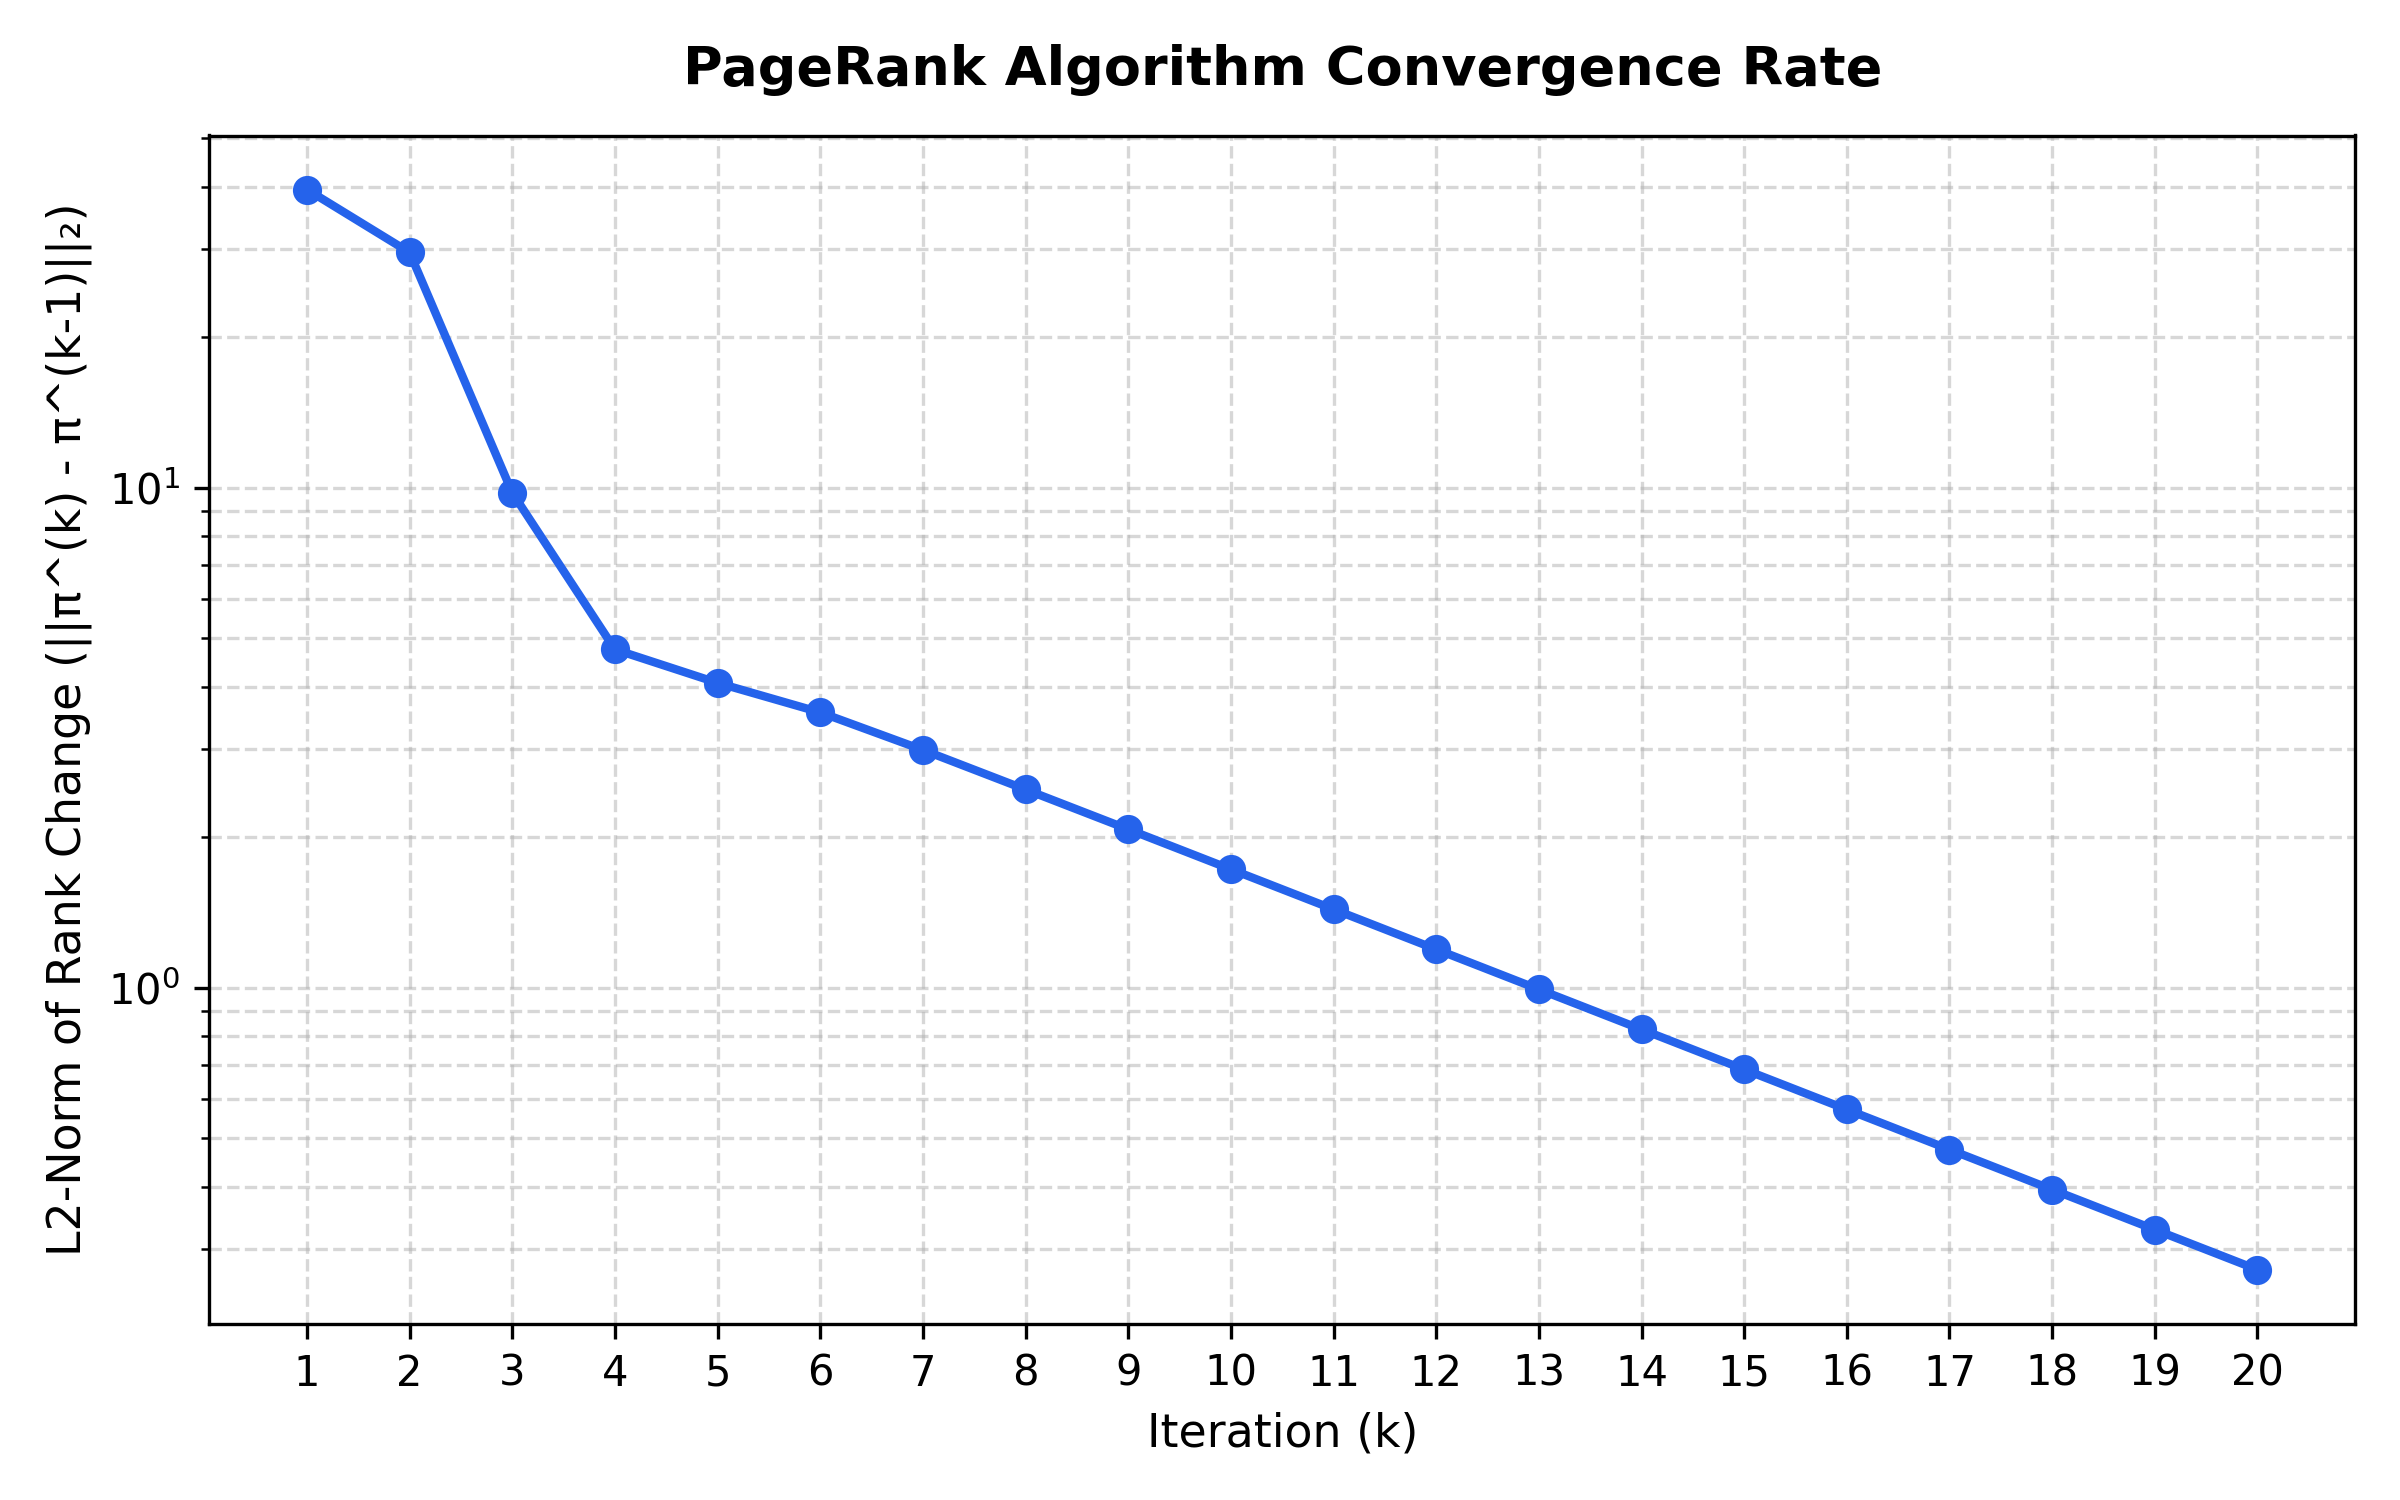
\includegraphics[width=0.8\textwidth]{Figures/pagerank_convergence.png}
    \caption{PageRank convergence rate over iterations calculated on the football transfer network.}
    \label{fig:pagerank_convergence}
\end{figure}


\subsubsection{Limitations of the Classical Model}

Despite its elegance, classical PageRank has notable limitations~\cite{cornell_limitations, wairimu_limitations}:

\begin{itemize}
    \item \textbf{Uniform Teleportation:} The standard model teleports users uniformly across the web, ignoring personalized contexts or specific user intents.
    \item \textbf{Equal Link Weighting:} It assumes all outgoing links have equal semantic value, dividing rank blindly by out-degree.
    \item \textbf{Vulnerability to Manipulation:} The algorithm is highly susceptible to artificial ``link farms'' created by malicious actors to inflate rankings.
    \item \textbf{Bias Against New Nodes:} Older nodes accumulate more links over time, making it difficult for newly created, highly relevant nodes to surface quickly.
\end{itemize}


%-------------------------------------------------------------
\subsection{The HITS Algorithm}
\label{subsec:hits}

While PageRank evaluates the web as a single, uniform landscape, the Hyperlink-Induced Topic Search (HITS) algorithm, developed by Jon Kleinberg in 1999, takes a fundamentally different, query-dependent approach. Instead of assigning a single rank to a page, HITS recognizes that web pages serve two distinct semantic functions: providing information or providing directions~\cite{kleinberg1999hits}.

Consequently, HITS assigns two separate scores to every node in the network:

\begin{itemize}
    \item \textbf{Authority Score} ($a$): Measures the quality and relevance of the information on a page. A good Authority is a page that is linked to by many good Hubs.
    \item \textbf{Hub Score} ($h$): Measures the quality of the links provided by a page. A good Hub is a page that links to many good Authorities.
\end{itemize}

This creates a mutually reinforcing relationship: a node's authority depends on the hubs pointing to it, and its hub value depends on the authorities it points to~\cite{kleinberg1999hits}.


\subsubsection{Mathematical Formulation of HITS}

The HITS algorithm computes these scores iteratively using a pair of update equations. For a given node $v$ in a directed graph $G = (V,E)$:

\noindent\textbf{The Authority Update Rule:}
\begin{equation}
\label{eq:hits_authority}
a(v) = \sum_{u \in B_v} h(u)
\end{equation}
where:
\begin{itemize}
    \item $a(v)$: The Authority score of node $v$.
    \item $B_v$: The set of all nodes $u$ that point to node $v$ (in-links).
    \item $h(u)$: The Hub score of the incoming node $u$.
\end{itemize}

\noindent\textbf{The Hub Update Rule:}
\begin{equation}
\label{eq:hits_hub}
h(v) = \sum_{w \in F_v} a(w)
\end{equation}
where:
\begin{itemize}
    \item $h(v)$: The Hub score of node $v$.
    \item $F_v$: The set of all nodes $w$ that node $v$ points to (out-links).
    \item $a(w)$: The Authority score of the destination node $w$.
\end{itemize}

Because these scores are continually added together during each iteration, the numbers can quickly grow to infinity. To solve this, HITS requires a \textbf{Normalization} step at the end of every iteration. Both the hub and authority scores of all nodes are divided by the sum (or the square root of the sum of squares) of all scores in the network, ensuring the values remain stable and converge~\cite{kleinberg1999hits, ijarcce_comparative}.


\subsubsection{Matrix Interpretation}

The HITS update rules can be expressed in matrix form. Let $\mathbf{A}$ be the $N \times N$ adjacency matrix of the directed graph, where $A_{ij} = 1$ if there is an edge from node $i$ to node $j$. Let $\mathbf{a}$ and $\mathbf{h}$ denote the authority and hub score vectors, respectively. Then the update rules become~\cite{kleinberg1999hits}:
\begin{equation}
\label{eq:hits_matrix_update}
\mathbf{a}^{(k+1)} = \mathbf{A}^{T}\,\mathbf{h}^{(k)}, \qquad \mathbf{h}^{(k+1)} = \mathbf{A}\,\mathbf{a}^{(k+1)}
\end{equation}

Substituting the first equation into the second yields:
\begin{equation}
\label{eq:hits_eigenvector}
\mathbf{a}^{(k+1)} = \mathbf{A}^{T}\mathbf{A}\,\mathbf{a}^{(k)}, \qquad \mathbf{h}^{(k+1)} = \mathbf{A}\mathbf{A}^{T}\,\mathbf{h}^{(k)}
\end{equation}

Thus, the authority vector converges to the principal eigenvector of $\mathbf{A}^{T}\mathbf{A}$, and the hub vector converges to the principal eigenvector of $\mathbf{A}\mathbf{A}^{T}$~\cite{kleinberg1999hits}. These are, equivalently, the left and right singular vectors of $\mathbf{A}$ corresponding to the largest singular value, establishing a deep connection between HITS and singular value decomposition (SVD)~\cite{ijarcce_comparative}.


\subsubsection{Operational Procedure}

Unlike PageRank, which is computed over the entire web graph offline, HITS operates on a focused subgraph constructed in response to a specific user query. The operational procedure consists of three phases~\cite{kleinberg1999hits}:

\begin{enumerate}
    \item \textbf{Root Set Construction:} A traditional text-based search engine returns a set of pages relevant to the query. This is the \textit{root set} $R$.
    \item \textbf{Base Set Expansion:} The root set is expanded to include all pages that either link to or are linked from any page in $R$, forming the \textit{base set} $S \supseteq R$.
    \item \textbf{Iterative Computation:} The hub and authority scores are iteratively computed over the subgraph induced by $S$ until convergence.
\end{enumerate}


%-------------------------------------------------------------
\subsection{Modified PageRank Variants}
\label{subsec:pagerank_variants}

To address the shortcomings of the classical PageRank model enumerated in Section~\ref{subsec:pagerank}, researchers have developed advanced variants:

\begin{itemize}
    \item \textbf{Personalized PageRank (PPR):} Replaces the uniform teleportation vector with a custom probability distribution vector tailored to individual user interests, confining rank to a specific topological neighborhood~\cite{personalized_pagerank}. Formally, the teleportation component $\frac{1-d}{N}$ is replaced by $(1-d) \cdot \mathbf{p}$, where $\mathbf{p}$ is a personalization vector with $\|\mathbf{p}\|_1 = 1$.

    \item \textbf{Topic-Sensitive PageRank:} Uses precomputed rank vectors biased toward representative basis topics. It calculates a query-sensitive score using a linear combination of these topic-specific ranks to improve precision~\cite{topic_sensitive_pagerank}. Given $K$ topic categories, $K$ separate PageRank vectors $\{\boldsymbol{\pi}_1, \dots, \boldsymbol{\pi}_K\}$ are precomputed, and at query time, the final score is $\boldsymbol{\pi}_q = \sum_{j=1}^{K} c_j \boldsymbol{\pi}_j$, where the coefficients $c_j$ reflect the query's topical distribution.

    \item \textbf{Weighted PageRank (WPR):} Replaces equal link division by allocating rank dynamically based on the relative popularity (in-links and out-links) of the destination nodes~\cite{weighted_pagerank_geeks, weighted_pagerank_trec}. This variant is of particular relevance to the present thesis, as the football transfer network inherently possesses weighted edges corresponding to transfer fees.

    \item \textbf{TrustRank:} Combats link spam by propagating trust outward from a rigorously vetted ``seed set'' of highly reputable nodes, neutralizing artificially inflated rank structures~\cite{trustrank2004}.
\end{itemize}


%-------------------------------------------------------------
\subsection{Distributed Graph Processing}
\label{subsec:distributed_graph}

Real-world graphs---the web graph, social networks, and large-scale transaction networks---routinely contain billions of nodes and edges, far exceeding the memory and computational capacity of a single machine. Distributed graph processing frameworks address this challenge by partitioning the graph across a cluster of machines and executing algorithms in parallel, with inter-machine communication for edge-boundary updates~\cite{spark_graphx, pregel2010}.

The two dominant programming models for distributed graph processing are:

\begin{enumerate}
    \item \textbf{Bulk Synchronous Parallel (BSP):} Exemplified by Google's Pregel~\cite{pregel2010} and Apache Giraph, BSP organizes computation into a sequence of \textit{supersteps}. In each superstep, every vertex executes a user-defined function, sends messages to its neighbors, and synchronizes with all other vertices before the next superstep begins.

    \item \textbf{MapReduce-Based Models:} Exemplified by Apache Spark's GraphX~\cite{spark_graphx}, these models express graph algorithms as sequences of distributed data transformations (map, filter, join, reduce) over vertex and edge tables, leveraging the in-memory caching and fault tolerance of the underlying dataflow engine.
\end{enumerate}


%-------------------------------------------------------------
\subsection{Apache Spark and GraphX}
\label{subsec:spark_graphx}

Apache Spark is an open-source, general-purpose distributed computing framework designed for large-scale data processing~\cite{spark_graphx}. Its core abstraction is the \textbf{Resilient Distributed Dataset (RDD)}, an immutable, partitioned collection of objects that can be operated on in parallel across a cluster. Spark extends the MapReduce model with in-memory caching, enabling iterative algorithms---such as PageRank and HITS---to avoid the costly disk I/O that hampers Hadoop MapReduce performance~\cite{spark_graphx}.

\textbf{GraphX} is Spark's library for graph-parallel computation. It extends the RDD abstraction with a \textbf{Graph} object, composed of a vertex RDD and an edge RDD, and provides a set of fundamental graph operators (\texttt{mapVertices}, \texttt{mapEdges}, \texttt{subgraph}, \texttt{joinVertices}, \texttt{aggregateMessages}) and optimized implementations of common graph algorithms, including PageRank~\cite{spark_graphx}.

The \textbf{PySpark} API exposes Spark's functionality through Python, enabling the implementation of custom graph algorithms using Spark's distributed DataFrames and RDDs without requiring Scala or Java. For this thesis, PySpark serves as the primary implementation language, enabling seamless integration with a Python-based web application backend.

The key architectural properties of Spark that make it well-suited for iterative graph algorithms include:

\begin{itemize}
    \item \textbf{In-Memory Computation:} Intermediate results from each iteration are cached in memory, eliminating redundant disk reads and dramatically accelerating iterative convergence~\cite{spark_graphx}.
    \item \textbf{Lazy Evaluation:} Transformations are recorded as a lineage graph (DAG) and executed only when an action triggers materialization, enabling Spark's optimizer to plan efficient execution strategies.
    \item \textbf{Fault Tolerance:} Lost partitions are automatically recomputed from the lineage DAG, without requiring explicit checkpointing for short computations.
    \item \textbf{Horizontal Scalability:} The framework scales linearly by adding worker nodes to the cluster, enabling the processing of arbitrarily large graphs.
\end{itemize}


%-------------------------------------------------------------
\subsection{Complex Network Applications}
\label{subsec:complex_networks}

Beyond web search, PageRank is instrumental in modeling complex socioeconomic ecosystems. The mathematical generality of link analysis algorithms---requiring only a directed graph as input---permits their application to any domain in which entities and directed relationships can be identified~\cite{liu2014football, ieice2016football, employee_arxiv}.

\subsubsection{Football Player Transfer Networks}

The professional football transfer market can be formally modeled as a directed graph $G_{FTN}=(V,E,W)$, where nodes $V$ are clubs, edges $E$ are player transfers, and the weight matrix $W$ represents monetary transfer fees. Evaluating this weighted network via PageRank measures a club's global ``coreness'' and systemic market competitiveness. High PageRank centrality correlates strongly with a club's ability to attract top-tier talent and its eventual on-pitch performance~\cite{liu2014football, ieice2016football}.

To accurately model this financial dynamic, the standard algorithm is adapted into a Weighted PageRank formula:
\begin{equation}
\label{eq:weighted_pagerank}
PR(u) = (1-d) + d \sum_{v \in B_u} \left( PR(v) \times \frac{W(v,u)}{\displaystyle\sum_{w \in F_v} W(v,w)} \right)
\end{equation}

Where the variables are defined as follows:
\begin{itemize}
    \item $PR(u)$: The new PageRank score of the destination club $u$ (the Buyer).
    \item $d$: The Damping Factor. In standard implementations, this is 0.85. It represents the probability that the algorithm continues following links rather than jumping randomly.
    \item $(1-d)$: The Teleportation baseline. In standard implementations, this is 0.15. It guarantees every club gets a baseline score of 0.15 per iteration so no club drops entirely to zero.
    \item $B_u$: The set of all clubs that link to club $u$ (all clubs that sold a player to club $u$).
    \item $PR(v)$: The current PageRank score of the source club $v$ (the Seller).
    \item $W(v,u)$: The mathematical Weight (Transfer Fee) assigned to the specific edge between club $v$ and club $u$.
    \item $\displaystyle\sum_{w \in F_v} W(v,w)$: The sum of all outgoing weights from club $v$. (The total amount of transfer fees club $v$ received across all its sales).
\end{itemize}


\subsubsection{Employee Mobility Networks}

Similarly, corporate ecosystems can be modeled as employee mobility networks $G_{EMN}=(V,E,W)$, where nodes are companies and edges represent employee migration. Edges can be weighted by proxy metrics like seniority gains or salary. In this context, PageRank identifies organizations with maximal global competitiveness. High-PageRank firms benefit disproportionately from systemic knowledge spillovers, successfully attracting strategic human capital and industry trade secrets~\cite{employee_arxiv, employee_econstor, employee_duke}.


%=============================================================
\section{Literature Review}
\label{sec:literature_review}

%-------------------------------------------------------------
\subsection{PageRank: Origins and Evolution}
\label{subsec:lit_pagerank}

The PageRank algorithm was first formally described by Brin and Page in their seminal 1998 paper, ``The Anatomy of a Large-Scale Hypertextual Web Search Engine''~\cite{brin1998pagerank}. The original formulation was subsequently refined in the Stanford InfoLab technical report, which provided a detailed mathematical treatment of the convergence properties of the power iteration method and the spectral properties of the Google Matrix~\cite{stanford1999pagerank}. The algorithm's elegant reduction of the web ranking problem to a well-understood problem in linear algebra---computing the principal eigenvector of a stochastic matrix---was instrumental in establishing Google as the dominant search engine of the early 2000s.

Subsequent research explored the sensitivity of PageRank to the damping factor. Boldi et al.\ demonstrated that while $d = 0.85$ yields good empirical results for web search, the choice of $d$ fundamentally governs the tradeoff between the influence of the global teleportation component and the local link structure. Higher values of $d$ increase the weight placed on link structure but slow convergence~\cite{york_lecture_slides}.

Langville and Meyer provided a comprehensive linear-algebraic treatment of PageRank, situating it within the broader theory of Markov chains and connecting it to classical results in matrix analysis. Their work clarified the relationship between the spectral gap of the Google Matrix and the convergence rate of the power iteration, establishing that the number of iterations required for convergence scales as $O(\log(N)/\log(1/d))$~\cite{pagerank_wikipedia}.

The study of PageRank on networks with special topological properties has also attracted significant attention. Csat\'o and T\'oth analyzed the behavior of PageRank on ``gluing networks''---graphs formed by connecting smaller component graphs---and derived analytic expressions for the PageRank distribution in terms of the component structures~\cite{mdpi_gluing}.


%-------------------------------------------------------------
\subsection{HITS: Hubs, Authorities, and Query-Dependent Analysis}
\label{subsec:lit_hits}

Kleinberg's 1999 paper, ``Authoritative Sources in a Hyperlinked Environment''~\cite{kleinberg1999hits}, introduced the HITS algorithm as an alternative to the global ranking paradigm of PageRank. The key conceptual innovation was the recognition that web pages serve distinct structural roles---some pages are primarily repositories of authoritative content, while others function as curated directories (hubs) that aggregate links to authoritative pages.

The HITS algorithm's query-dependent nature represented both its principal strength and its primary limitation. By restricting computation to a focused subgraph relevant to a specific query, HITS could deliver more topically precise results than a global ranking~\cite{kleinberg1999hits}. However, this same restriction made the algorithm vulnerable to \textit{topic drift}---the phenomenon whereby a small number of densely connected but off-topic nodes dominate the subgraph and distort the authority and hub scores~\cite{ijarcce_comparative, ijca_hits_pagerank_2024}.

Bharat and Henzinger provided an early empirical analysis of HITS and identified the topic drift problem, proposing mitigations that included weighting the edges of the base set by the textual similarity between the linked pages. Subsequent work by Chakrabarti et al.\ proposed extensions that combined link analysis with content analysis to improve the topical coherence of HITS results~\cite{ijarcce_comparative}.


%-------------------------------------------------------------
\subsection{Comparative Studies of PageRank and HITS}
\label{subsec:lit_comparative}

The comparative analysis of PageRank and HITS has been the subject of numerous studies spanning over two decades. The key dimensions of comparison that emerge from the literature are execution model, graph scope, computational cost, vulnerability to manipulation, and output semantics.

Duhan and Sharma provided one of the earliest comprehensive comparative surveys, systematically contrasting the two algorithms on the dimensions of computation time, spam resilience, and query dependence. Their analysis concluded that PageRank's offline, global computation makes it more robust to manipulation and more efficient at query time, while HITS provides richer structural information but at the cost of increased latency and spam vulnerability~\cite{ijarcce_comparative}.

A comparative study published in the International Journal of Advanced Research in Computer and Communication Engineering (IJARCCE)~\cite{ijarcce_comparative} evaluated both algorithms on synthetic and real-world web graph datasets, confirming that PageRank demonstrates superior stability across varying graph topologies, while HITS excels in identifying topically coherent clusters of hubs and authorities. The study further noted that the dual hub--authority decomposition of HITS provides information that is fundamentally inaccessible to PageRank, which collapses all structural roles into a single scalar score.

Research published in the International Journal of Engineering Research and Technology (IJERT)~\cite{ijert_comparative} extended the comparison to include computational scalability, demonstrating that while both algorithms have comparable asymptotic complexity per iteration---$O(N + E)$---HITS incurs additional overhead due to the base set expansion step and the need for two-phase (hub and authority) updates per iteration. However, the smaller size of the HITS subgraph relative to the full web graph typically more than compensates for this per-iteration overhead.

A more recent comparative analysis published in the International Journal of Computer Applications (IJCA) in 2024~\cite{ijca_hits_pagerank_2024} revisited the comparison in the context of modern web architectures, which are characterized by dynamic content, social media integration, and mobile-first design. The study argued that neither algorithm in its classical form is sufficient for contemporary web ranking, but that their underlying principles---global topological authority (PageRank) and local hub--authority decomposition (HITS)---remain foundational building blocks for modern hybrid ranking systems.


%-------------------------------------------------------------
\subsection{Distributed Implementations of Link Analysis}
\label{subsec:lit_distributed}

The need to compute PageRank and HITS on web-scale graphs motivated the development of distributed implementations from the earliest days of both algorithms. The original PageRank computation at Google was implemented on a distributed cluster of commodity machines using a custom MapReduce-like framework~\cite{brin1998pagerank}.

The advent of Apache Hadoop's MapReduce provided the first widely accessible platform for distributed PageRank computation. However, the repeated reading and writing of intermediate results to disk between MapReduce jobs made Hadoop poorly suited for the iterative nature of both PageRank and HITS~\cite{spark_graphx}.

Apache Spark's introduction of in-memory RDDs represented a transformative improvement for iterative graph algorithms. Gonzalez et al.\ demonstrated that Spark's GraphX library could compute PageRank on web-scale graphs up to $100\times$ faster than Hadoop-based implementations, primarily due to the elimination of inter-iteration disk I/O. The GraphX programming model expresses graph algorithms as sequences of join and aggregation operations on vertex and edge tables, which the Spark optimizer can parallelize and pipeline efficiently~\cite{spark_graphx}.


%-------------------------------------------------------------
\subsection{Graph Analytics in Non-Web Domains}
\label{subsec:lit_nonweb}

The application of link analysis algorithms to non-web domains has expanded dramatically over the past two decades, reflecting the growing recognition that many real-world systems can be productively modeled as directed graphs.

\subsubsection{Football Transfer Networks}

Liu et al.\ were among the first to apply network analysis techniques to the football transfer market, constructing a directed graph of transfers among European clubs and computing various centrality measures, including PageRank~\cite{liu2014football}. Their analysis revealed a core--periphery structure in the transfer network, with a small number of elite clubs (e.g., Manchester United, Real Madrid, FC Barcelona) forming a densely interconnected core that disproportionately attracts talent from a larger periphery of lower-ranked clubs. Subsequent studies published in PMC~\cite{liu2014football}, IEICE Transactions~\cite{ieice2016football}, and ResearchGate~\cite{football_researchgate} corroborated these findings and extended them to include temporal dynamics, demonstrating that the transfer network evolves over time in response to regulatory changes, financial fair play rules, and economic shocks.

\subsubsection{Employee Mobility Networks}

A parallel line of research has applied graph-theoretic methods to the analysis of employee mobility between firms. Studies published on arXiv~\cite{employee_arxiv}, EconStor~\cite{employee_econstor}, and the Duke Economics Working Paper series~\cite{employee_duke} have modeled inter-firm employee flows as directed graphs and used PageRank and related centrality measures to identify firms that function as ``talent magnets'' or ``talent exporters'' within an industry ecosystem. High-PageRank firms in these networks have been shown to correlate with superior financial performance, innovation output, and market valuation, suggesting that the ability to attract human capital is both a cause and consequence of organizational success.


%=============================================================
\section{Datasets}
\label{sec:datasets}

The primary dataset employed in this thesis is a comprehensive record of professional football player transfers across major European leagues. The dataset encompasses multiple seasons and leagues, including the English Premier League, La Liga (Spain), Serie A (Italy), Bundesliga (Germany), Ligue~1 (France), Liga NOS (Portugal), Eredivisie (Netherlands), the Jupiler Pro League (Belgium), the English Championship, and several other national and international competitions.

Each record in the dataset corresponds to an individual transfer event and contains the fields described in Table~\ref{tab:dataset_fields}.

\begin{table}[htbp]
\centering
\caption{Dataset fields and their roles in the graph construction.}
\label{tab:dataset_fields}
\begin{tabular}{l l l}
\hline
\textbf{Field} & \textbf{Description} & \textbf{Role in Graph} \\
\hline
Selling Club   & The club transferring the player out     & Source node       \\
Buying Club    & The club acquiring the player             & Destination node  \\
Transfer Fee (\euro) & The monetary amount of the transfer & Edge weight       \\
Season         & The football season of the transfer       & Temporal filter   \\
League         & The league of the buying/selling club     & Categorical filter\\
Player Name    & The name of the transferred player        & Edge metadata     \\
\hline
\end{tabular}
\end{table}

The graph is constructed by aggregating individual transfer records into a directed edge list. Each unique club constitutes a node. A directed edge from club $v$ to club $u$ indicates that club $v$ sold at least one player to club $u$. In the weighted variant, the edge weight $W(v, u)$ is the total monetary value (in euros) of all transfers from $v$ to $u$ within the selected time window.

The dataset supports multiple filtering dimensions---by league, by season range, and by weighting mode (transfer fee in euros or unweighted transfer count)---enabling the user to analyze the graph structure under varying conditions.


%=============================================================
\section{Evaluation Metrics}
\label{sec:eval_metrics_bg}

The comparative evaluation of PageRank and HITS in this thesis employs the following metrics and analytical dimensions:

\textbf{1.\ Rank Score Distribution.} For PageRank, we analyze the distribution of the scalar PageRank scores $PR(v)$ across all nodes. For HITS, we separately analyze the distributions of authority scores $a(v)$ and hub scores $h(v)$. Visualization via ranked bar charts enables direct identification of the top-$N$ nodes by each score.

\textbf{2.\ Rank Correlation.} To quantify the agreement or disagreement between the rankings produced by PageRank and HITS (authority), we employ Spearman's rank correlation coefficient $\rho$, defined as:
\begin{equation}
\label{eq:spearman}
\rho = 1 - \frac{6 \sum_{i=1}^{N} d_i^2}{N(N^2 - 1)}
\end{equation}
where $d_i$ is the difference between the rank of node $i$ under PageRank and its rank under HITS authority. A value of $\rho = 1$ indicates perfect agreement, $\rho = 0$ indicates no correlation, and $\rho = -1$ indicates perfect inversion.

\textbf{3.\ Hub--Authority Asymmetry.} HITS uniquely provides two scores per node, enabling the identification of nodes that function primarily as hubs (high $h$, low $a$) or primarily as authorities (high $a$, low $h$). This asymmetry is not captured by PageRank and constitutes a qualitative advantage of HITS for structural role analysis.

\textbf{4.\ Convergence Rate.} For a fixed tolerance threshold $\epsilon$, the number of iterations required for each algorithm to converge provides a measure of computational efficiency. In the context of our implementation, the user configures a fixed number of iterations (default: 10), and the stability of scores across the final iterations indicates the degree of convergence achieved.

\textbf{5.\ Sensitivity to Parameters.} The sensitivity of each algorithm's output to configurable parameters---damping factor $d$ for PageRank, iteration count $k$ for both algorithms, and weighting mode (fee-weighted vs.\ unweighted) for both algorithms---provides insight into the robustness and stability of the rankings.

\textbf{6.\ Network Topology Metrics.} Complementary graph metrics---including in-degree centrality, out-degree centrality, betweenness centrality, and clustering coefficient---provide context for interpreting the PageRank and HITS scores and assessing the extent to which the algorithmic rankings capture structural properties beyond simple degree.


%=============================================================
\section{Discussion}
\label{sec:bg_discussion}

The literature reviewed in the preceding sections reveals several key themes that inform the design of the comparative study presented in this thesis.

First, \textbf{PageRank and HITS embody fundamentally different philosophies of ranking}. PageRank computes a single, global, query-independent importance score that reflects a node's overall centrality in the entire network. HITS computes two query-dependent scores that capture the distinct structural roles of hubs and authorities within a localized subgraph. These philosophies are complementary rather than competing: PageRank answers the question ``How globally important is this node?'' while HITS answers the question ``What role does this node play in this specific context?''~\cite{ijarcce_comparative, ijert_comparative, ijca_hits_pagerank_2024}.

Second, \textbf{the mathematical formulations of both algorithms are grounded in spectral graph theory}. PageRank is the principal eigenvector of the Google Matrix; HITS authority and hub vectors are the principal eigenvectors of $\mathbf{A}^{T}\mathbf{A}$ and $\mathbf{A}\mathbf{A}^{T}$, respectively. This shared spectral foundation enables a unified theoretical treatment while highlighting the structural differences in the matrices involved~\cite{stanford1999pagerank, kleinberg1999hits}.

Third, \textbf{distributed implementation is essential for scalability}. Both algorithms are inherently iterative, requiring repeated global communication (rank propagation) across the graph. Apache Spark's in-memory computation model, combined with GraphX's graph-parallel operators, provides an efficient and scalable platform for both algorithms~\cite{spark_graphx, elmaddah_project}.

Fourth, \textbf{non-web domains provide fertile ground for link analysis}. The football transfer network, employee mobility networks, and other socioeconomic graphs exhibit structural properties---such as core--periphery organization, heavy-tailed degree distributions, and community structure---that are well-suited to analysis via PageRank and HITS~\cite{liu2014football, ieice2016football, employee_arxiv, employee_econstor, employee_duke}.

Finally, \textbf{a significant gap exists in the availability of unified, interactive tools} that enable side-by-side comparison of PageRank and HITS on the same dataset under identical conditions, with configurable parameters and multiple visualization modalities. The Transfer Analyzer application developed in this thesis is designed to fill precisely this gap.
